\section{Ergebnisse}
Zunächst wurden bei einer Belichtungszeit von 30 Sekunden dark frames bei verschiedenen Temperaturen des Chips aufgenommen, um die ideale Betriebstemperatur des CCD zu ermitteln. Hierbei ergaben sich die in Tabelle \ref{tbl:adu_temp} dargestellten Werte, welche in Abb. \ref{fig:adu_temp} graphisch dargestellt sind. 
\begin{figure}[h!]
        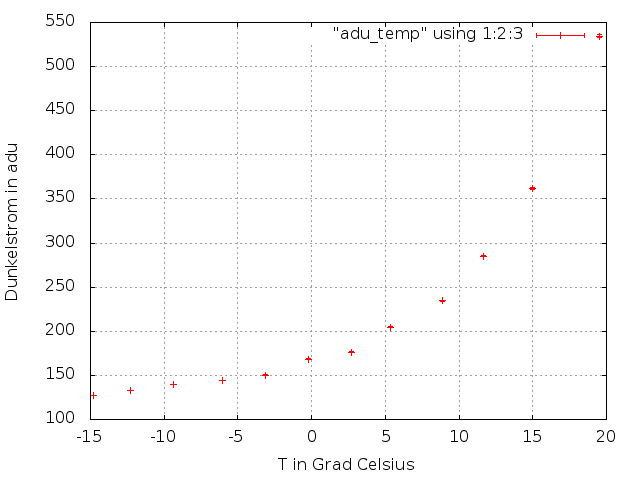
\includegraphics[width=.9\textwidth]{plot_adu_temp.png}
\caption{ Auftragung von Dunkelstrom über der CCD-Temperatur }
\label{fig:adu_temp}
\end{figure}
Hier wurde der Verlauf mit einer Exponentialfunktion $f(T) = a \cdot \exp(T \cdot c) + b$ gefittet, welche theoretisch zu erwarten ist, da die Energie der Elektronen im Halbleiter prinzipiell boltzmann-verteilt ist. \\
Es ergibt sich also eine ideale Temperatur von etwa -15 $^\circ$ C im betrachteten Intervall von -15 bis + 20 $^\circ$ C. Eine tiefere Temperatur ist aufgrund der begrenzten Kühlleistung des CCD-Chips nicht erreichbar. Für die Fitparameter ergibt sich: 
$a = 40.0\  \mathrm{adu}, c = 0.119 \frac{1}{\mathrm{K}}, b = 124.2 \ \mathrm{adu}$. \\
Die Aufnahme eines bias frames bei einer Belichtungszeit von 0.12 s und einer Blendenöffnung von 5.6 wird in Abb. \ref{fig:bias} dargestellt. 
\begin{figure}[h!]
        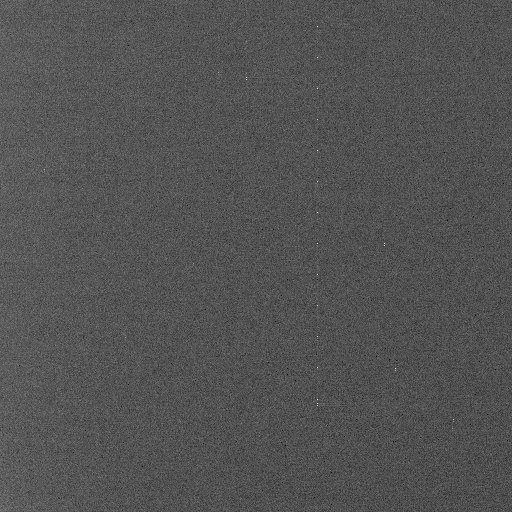
\includegraphics[width=.9\textwidth]{beiers_01.png}
\caption{ Aufnahme eines bias frame }
\label{fig:bias}
\end{figure}
Neben dem Rauschen im Hintergrund erkennt man mehrere senkrechte gepunktete Linien. Diese sind auf ein hot pixel in der entsprechenden Spalte zurückzuführen. Aufgrund des \enquote{schubweisen} Auslesens der Zeilen, welches  laut dem Betreuer durch Speichervorgänge in der Ausleseelektronik verursacht wird, kommt es in regelmäßigen zeitlichen Abständen zu einer Verzögerung beim Auslesen und somit zu hellen Punkten mit räumlich gleichem Abstand. Des weiteren ist ein leichter Helligkeitsgradient von links nach rechts sichtbar. Der Grund hierfür ist wahrscheinlich ein Temperaturgradient im CCD-Chip und ein somit räumlich unterschiedlicher Dunkelstrom. \\
Es wurden insgesamt 11 bias frames aufgenommen, deren mittlerer ADU-Wert sich zu 115.6 $ \pm 1.07$ ergibt. \\
Zur Bestimmung des Gain-Faktors werden zu jeder Belichtungsdauer je zwei flat fields aufgenommen und ausgewertet. Dabei ergeben sich mit der Formel ... die in Tabelle \ref{tbl:gain} dargestellten Werte. Als gemittelter Wert ergibt sich 
\begin{equation}
\bar{g} = 1.940 \pm 0.04 \ \frac{\mathrm{adu}}{\mathrm{e}}. 
\end{equation}
Die Werte für den Gain-Faktor sind zwar alle im gleichen Bereich, für eine kürzere Belichtungszeit ergibt sich allerdings ein größerer Gain-Faktor. Grund???\\
In Tabelle \ref{tbl:adu_int} sind die Werte für gemessenen ADU-Werte aufgetragen über dem durch die Filter transmittierten Licht als Anteil der Intensität vor dem Filter. 
